% =====================================================================
% Artigo — Análise e Projeto de Algoritmos (Unisinos, 2026/2)
% Template SBC da professora (sbc-template.sty + sbc.bst).
%
% COMO USAR
%  - \lacuna{...} = texto a escrever pelo grupo (aparece em vermelho no PDF).
%    Antes de entregar: procurar "\lacuna" e garantir que não sobrou nenhuma.
%  - Comentários "% MATERIAL:" = lembretes curtos (números, fontes, onde está
%    no roteiro). Não aparecem no PDF. Detalhes em Artigo/artigo/artigo-poda.md.
%  - Tabelas e figuras já estão com os dados finais (CSVs do Rodrigo, 3bb29f7).
%  - Limite: 10 a 15 páginas. Entrega: 23/11/2026, 19h30, Moodle.
% =====================================================================
\documentclass[12pt]{article}

\usepackage{sbc-template}
\usepackage{graphicx,url}
\usepackage[T1]{fontenc}
\usepackage[utf8]{inputenc}
\usepackage[brazilian]{babel}
\usepackage{booktabs}
\usepackage{amsmath}
\usepackage{xcolor}
\usepackage{placeins}
\usepackage{float}

\graphicspath{{figuras/}}

% Lacuna: texto do grupo ainda não escrito
\newcommand{\lacuna}[1]{\textcolor{red}{[#1]}}

\sloppy

\title{Análise do Impacto das Estratégias de Poda no Desempenho de Algoritmos de Busca: Um Estudo sobre os Problemas do Caixeiro Viajante e das N Rainhas}

\author{Rodrigo Mello\inst{1}, Vinicius de Avila Bezerra\inst{1}}

\address{Escola Politécnica -- Universidade do Vale do Rio dos Sinos (Unisinos)\\
  São Leopoldo -- RS -- Brasil
  \email{RodrigoMello2@edu.unisinos.br, BezerraVinicius@edu.unisinos.br}
}

\begin{document}

\maketitle

% MATERIAL: escrever por último. Até 10 linhas cada, ambos na primeira página.
% Pergunta do rascunho do Rodrigo: como diferentes estratégias de poda
% influenciam o desempenho de algoritmos de busca em problemas combinatórios.
\begin{abstract}
This study evaluates pruning strategies in N-Queens and Traveling Salesperson search. Brute force, Backtracking, and Branch and Bound were compared by explored nodes, pruning counts, and execution time (median of five runs after warm-up). For $N=8$, Backtracking reduced nodes from 19,173,961 to 2,057, while Branch and Bound was not always faster. For the 10-city TSP, Branch and Bound explored 855 nodes in 0.499 ms, versus 986,410 nodes and 19.0 ms for brute force. Results show pruning benefits depend on the problem. The study covers small inputs, one computer, and one TSP instance per size.
\end{abstract}

\begin{resumo}
Este estudo avalia estratégias de poda na busca das N Rainhas e do Caixeiro-Viajante. Foram comparados algoritmos de força bruta, Backtracking e Branch and Bound por nós explorados, podas e tempo (mediana de cinco execuções após aquecimento). Em $N=8$, o Backtracking reduziu os nós de 19.173.961 para 2.057, mas o Branch and Bound nem sempre foi mais rápido. No TSP com 10 cidades, o Branch and Bound explorou 855 nós em 0,499 ms, ante 986.410 nós e 19,0 ms da força bruta. Os resultados indicam que o benefício da poda varia conforme o problema. A avaliação limita-se a entradas pequenas, uma máquina e uma instância do TSP por tamanho.
\end{resumo}

% =====================================================================
\section{Introdução}
Problemas combinatórios frequentemente possuem um espaço de busca que cresce com o tamanho da entrada. Em muitos casos, encontrar uma solução exige considerar diferentes combinações de escolhas, o que pode tornar a enumeração completa computacionalmente custosa. Algoritmos de busca podem reduzir esse esforço por meio de estratégias de poda, que interrompem a exploração de estados inviáveis ou que não podem conduzir a uma solução melhor. Entretanto, identificar esses estados também exige operações adicionais; assim, uma poda pode reduzir o número de nós visitados sem necessariamente diminuir o tempo de execução.

Este trabalho examina esse equilíbrio em dois problemas com objetivos distintos. No problema das N rainhas, busca-se posicionar N peças em um tabuleiro sem que duas compartilhem a mesma coluna ou diagonal. Essas restrições permitem descartar posicionamentos parciais que já violem as condições do problema. No Problema do Caixeiro-Viajante (TSP), busca-se uma rota de menor custo que visite cada cidade uma única vez e retorne à origem; nesse caso, um limite inferior para o custo de uma rota parcial pode indicar que ela não levará a uma solução melhor que a já encontrada. A comparação permite observar como a natureza do problema influencia a estratégia de poda e seu custo.

A questão de pesquisa é: como diferentes estratégias de poda influenciam o desempenho computacional de algoritmos de busca aplicados a problemas combinatórios? O objetivo geral é analisar esse impacto considerando tanto a redução do espaço de busca quanto o custo das verificações realizadas. Para isso, são comparadas versões de força bruta, \textit{Backtracking} e \textit{Branch and Bound} aplicadas aos dois problemas. O desempenho é avaliado pelo tempo de execução, pelo número de nós explorados e pela quantidade de podas, e os resultados são relacionados à análise teórica da complexidade dos algoritmos.

O restante do artigo está organizado da seguinte forma: a Seção 2 apresenta os conceitos necessários e os problemas estudados; a Seção 3 descreve os algoritmos e o procedimento experimental; a Seção 4 analisa a complexidade; a Seção 5 apresenta os resultados; a Seção 6 discute sua relação com a análise teórica; e a Seção 7 conclui o trabalho, indicando limitações e possibilidades de continuidade.
% =====================================================================
\section{Fundamentação Teórica}

\subsection{Espaço de busca e busca exaustiva}

O espaço de busca reúne os estados que podem ser considerados na procura por soluções. Ele pode ser representado por uma árvore, na qual cada nó corresponde a um estado parcial e cada aresta, a uma decisão. A busca exaustiva percorre as alternativas possíveis até encontrar as soluções ou avaliar todo o espaço. Embora simples e útil como referência, pode se tornar custosa à medida que cresce o número de combinações. A enumeração de permutações, por exemplo, apresenta crescimento fatorial; já a atribuição de um entre n valores a cada uma de n posições gera $n^n$ possibilidades \cite{laaksonen:2018}.

\subsection{Backtracking e poda por restrição}

Backtracking constrói soluções de forma incremental e verifica, após cada escolha, se o estado parcial ainda pode ser estendido para uma solução válida. Se uma restrição já foi violada, a busca retrocede e deixa de explorar os estados descendentes. Por exemplo, nas N rainhas, uma escolha que viole as restrições do problema pode ser podada antes de completar o tabuleiro. Em problemas de satisfação de restrições, o \emph{forward checking} também verifica se as variáveis ainda não atribuídas mantêm valores compatíveis com as escolhas feitas \cite{haralick:1980}.

\subsection{Branch and Bound e poda por limite}

% "menor limite primeiro"; o nosso é em profundidade e sem solução inicial.
Branch and Bound é uma estratégia para problemas de otimização que divide o espaço em subproblemas e calcula um limite para a melhor solução que cada um pode conter. Em uma minimização, um subproblema pode ser podado quando seu limite não permite superar a melhor solução completa conhecida. Para preservar a correção, o limite deve ser otimista e não excluir soluções melhores. Na formulação de Little et al., os limites inferiores também orientam a ordem de exploração dos subproblemas \cite{little:1963}. Neste trabalho, a busca percorre a árvore em profundidade e usa um limite baseado em árvore geradora mínima, diferindo da exploração por menor limite primeiro descrita por esses autores.

\subsection{Problemas estudados}

O problema das N rainhas consiste em posicionar N rainhas em um tabuleiro N por N sem que duas se ataquem. Colocando uma rainha por linha, as escolhas podem ser verificadas quanto às restrições de coluna e diagonal. O estudo busca e conta configurações válidas, sem minimizar uma função de custo. O Problema do Caixeiro-Viajante (TSP), por sua vez, busca um ciclo de menor custo que visite cada cidade uma vez e retorne à origem. No caso simétrico, fixada a cidade inicial, percorrer o ciclo em sentidos opostos representa a mesma rota, resultando em (n-1)!/2 ciclos distintos. Uma árvore geradora mínima das cidades ainda não visitadas pode contribuir para um limite inferior do custo necessário para completar uma rota parcial; árvores geradoras mínimas e o algoritmo de Prim são tratados por Cormen et al. \cite{cormen:2012}.



% MATERIAL: 17 nós, 2 soluções (borda verde), 4 nós sem continuação (laranja);
% c/d = podas por coluna/diagonal. Força bruta: 341 nós em N=4.


% =====================================================================
\section{Metodologia}
% MATERIAL:
%  - 3 variantes por problema, mesma interface (NQueensSolver, TspSolver), mesmas instâncias.
%  - Métricas: tempo (System.nanoTime), nós, tentativas, podas por causa, avaliações do limite.
%  - Medição: por tamanho e solver (FB -> BT -> B\&B), 1 execução sem aquecimento
%    (warmup_elapsed_ns) + mediana de 5 com aquecimento (tempo_decorrido_ns).
%  - Só relatar o observado (primeira execução bem mais lenta); sem teoria da JVM.
%  - Tamanhos: N = 4..8; n = 2, 4, 6, 8, 10. TSP: semente 20261110 + n, pesos em [1, 100].
%  - Fig. 3: n=6, rota 0-1-4-2-3-5-0, custo 138.

O estudo compara, em Java, três algoritmos para cada problema: força bruta, Backtracking e Branch and Bound. Para as N Rainhas, são avaliados tabuleiros de tamanho N=4 a 8. A força bruta enumera as $N^N$ atribuições de colunas e valida as configurações completas; o Backtracking verifica incrementalmente as restrições de coluna e diagonal; e o Branch and Bound acrescenta um limite superior otimista para o número de linhas restantes que ainda podem receber uma rainha. Para o TSP, são usadas instâncias simétricas com n=2, 4, 6, 8 e 10 cidades. Os pesos inteiros das arestas variam de 1 a 100 e são gerados de forma determinística com a semente 20261110+n, permitindo que os três algoritmos recebam a mesma instância para cada tamanho. A força bruta enumera as rotas, o Backtracking evita estender prefixos com cidades já visitadas e o Branch and Bound poda rotas cujo limite inferior, calculado com uma árvore geradora mínima das cidades restantes e os custos de conexão, não pode melhorar a melhor rota completa encontrada. Nos três algoritmos do TSP, considera-se apenas uma das duas orientações equivalentes de cada ciclo.

O desempenho é avaliado pelo tempo de execução e por contadores de busca: nós explorados, tentativas de posicionamento ou inclusão de cidade, soluções completas avaliadas e podas discriminadas por causa. Também são contabilizadas as avaliações do limite e, nas N Rainhas, as configurações completas inválidas. O tempo é medido em nanossegundos com \texttt{System.nanoTime()}. Para cada tamanho e algoritmo, a execução inicial, utilizada como aquecimento, é cronometrada e armazenada separadamente. Em seguida, são realizadas cinco execuções medidas, e a mediana dos tempos é registrada. As execuções repetidas são verificadas quanto à consistência do número de soluções ou do custo ótimo; no TSP, também se valida que a rota visita cada cidade uma vez e retorna à origem. A instância ilustrada para n=6 possui rota ótima 0--1--4--2--3--5--0, de custo 138.

Os experimentos foram executados em um notebook com processador Intel Core i7-10510U
(1,80~GHz, 4 núcleos e 8 \emph{threads}), 15,8~GB de memória RAM (2.133~MT/s) e
Windows 11 Enterprise 10.0.26200 (64 bits). O equipamento permaneceu conectado à
energia, com o plano ``Equilibrado''. Foi utilizado o OpenJDK 21.0.10 (Microsoft Build).

% TODO: Corrigir link
O código-fonte do projeto está disponível no repositório:
\url{https://github.com/rodrigo-mello-hw08/unisinos-analise-e-projeto-algoritmos/tree/main/Artigo}.
\begin{figure}[htbp]
\centering
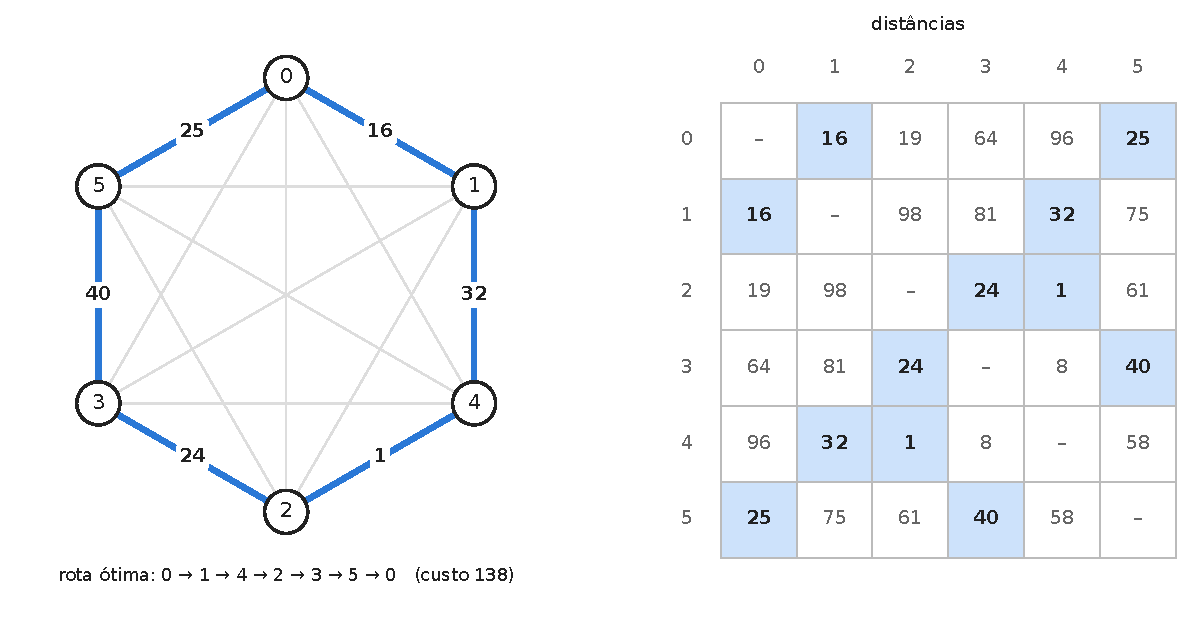
\includegraphics[width=\linewidth]{tsp-instancia-6.pdf}
\caption{\lacuna{legenda: instância do TSP com n=6 e rota ótima}}
\label{fig:tsp6}
\end{figure}

% =====================================================================


\begin{figure}[htbp]
\centering
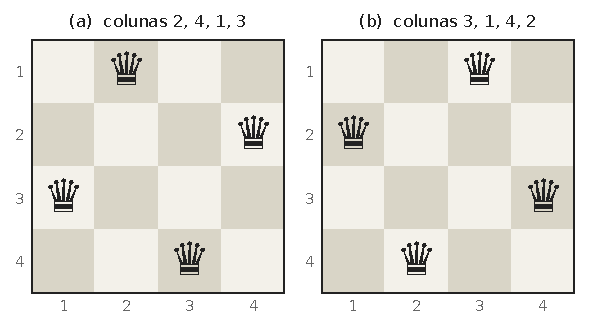
\includegraphics[width=.6\linewidth]{solucoes-rainhas-4.pdf}
\caption{\lacuna{legenda: as 2 soluções das N rainhas para N=4}}
\label{fig:solucoes4}
\end{figure}

\begin{figure}[htbp]
\centering
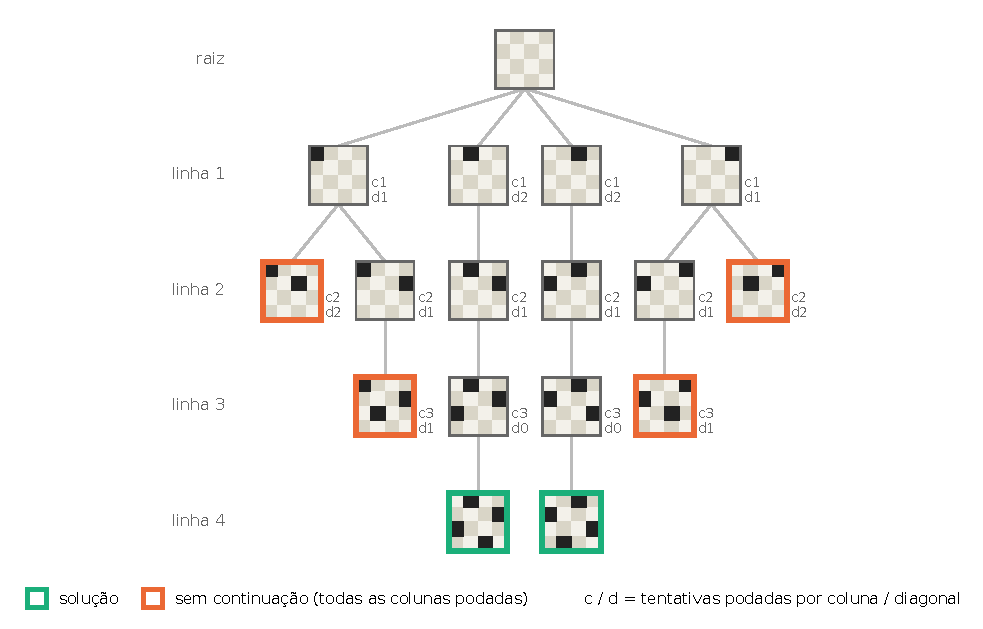
\includegraphics[width=\linewidth]{arvore-rainhas-4.pdf}
\caption{\lacuna{legenda: árvore de estados do backtracking, N=4}}
\label{fig:arvore4}
\end{figure}

\FloatBarrier

\section{Análise Teórica dos Algoritmos}

\subsection{N rainhas}

A análise considera o número de estados da árvore de busca e o trabalho realizado em cada estado. Na força bruta, cada uma das N linhas recebe uma coluna entre N opções, sem verificar conflitos até a configuração estar completa. Assim, o número de nós é
\[
V_{FB}(N)=\sum_{k=0}^{N}N^k=\frac{N^{N+1}-1}{N-1},\quad N>1.
\]
Há $N^N$ configurações completas, e a validação de cada uma compara pares de rainhas, custando $O(N^2)$. Portanto, o tempo é $O(N^N\,N^2)$, dominado pela validação das folhas.

No Backtracking, cada estado parcial usa no máximo uma coluna por linha, de modo que a árvore tem no máximo $\sum_{k=0}^{N}P(N,k)=O(N!)$ nós, onde $P(N,k)=N!/(N-k)!$. Na implementação, cada nó percorre até N colunas e testa em tempo constante as marcações de coluna e diagonais; logo, o tempo no pior caso é $O(N\,N!)$. A poda por restrição pode reduzir substancialmente a árvore efetivamente visitada, mas não altera esse limite superior.

O Branch and Bound das N Rainhas acrescenta, em cada estado não terminal, uma estimativa do número de linhas futuras que ainda possuem ao menos uma posição disponível. Essa avaliação percorre até N linhas e N colunas e custa $O(N^2)$ por nó. Como o número de nós não supera o da busca com as mesmas restrições, o pior caso é $O(N^2\,N!)$. A recorrência pode ser expressa como $T(k)=\sum_{j=1}^{N-k}T(k+1)+O(N^2)$, com custo constante nos estados completos; a soma explicita até $N-k$ chamadas recursivas possíveis e o custo do limite. Esse custo adicional pode não compensar quando a poda elimina poucos estados.

\subsection{Problema do Caixeiro-Viajante}

Com a cidade inicial fixada, a árvore do TSP possui até $n-1$ escolhas no primeiro nível, $n-2$ no seguinte e assim por diante. O número de nós é limitado por
\[
V(n)=\sum_{k=0}^{n-1}P(n-1,k)=O((n-1)!),
\]
onde k é o número de cidades adicionais no prefixo e $P(m,k)=m!/(m-k)!$. Cada nó percorre até n-1 cidades candidatas; além disso, o custo de uma rota completa é calculado em $O(n)$. Tanto a força bruta quanto o Backtracking têm, portanto, tempo de pior caso $O(n\,(n-1)!)$. Na implementação, ambos percorrem a mesma árvore de prefixos; a verificação de cidade visitada impede a recursão em candidatos repetidos, mas não reduz a ordem assintótica do número de nós. Como os custos são simétricos, a orientação canônica faz com que apenas $(n-1)!/2$ rotas completas sejam avaliadas, sem alterar a ordem do pior caso.

No Branch and Bound, cada estado não terminal calcula um limite inferior composto pelo custo parcial, por uma árvore geradora mínima das cidades ainda não visitadas e pelos custos mínimos de conexão com a cidade atual e com a origem. O algoritmo de Prim implementado por matriz de distâncias custa $O(n^2)$; assim, esse limite domina o percurso das candidatas em cada nó. No pior caso, nenhum limite elimina subárvores e o algoritmo visita $O((n-1)!)$ nós, resultando em $O(n^2\,(n-1)!)$. Em uma instância favorável, a poda pode diminuir o número de nós visitados, mas seu ganho depende de reduzir a árvore o bastante para compensar o cálculo do limite.

Em ambos os problemas, a recorrência de uma busca em profundidade pode ser escrita como $T(k)=b_kT(k+1)+c_k$, em que $b_k$ é o número máximo de escolhas que geram chamadas recursivas no nível k e $c_k$ é o custo local do estado, incluindo verificações e limites. A soma dos custos por nível corresponde à contagem de nós e ao trabalho executado em cada um, explicitando por que menor número de nós não implica necessariamente menor tempo.

% =====================================================================
\section{Experimentos e Resultados}
% TODO: Corrigir posicao das imagens
As três variantes produziram os mesmos resultados de correção para cada tamanho avaliado: o mesmo número de configurações válidas nas N Rainhas e o mesmo custo ótimo no TSP. A seção apresenta os nós explorados, as podas contabilizadas e os tempos de execução. Para o TSP, os resultados tabulados abrangem instâncias de 4, 6, 8 e 10 cidades; a instância de 2 cidades foi omitida por ser trivial.

A Tabela~\ref{tab:nos-rainhas} registra o número de soluções e de nós explorados para cada tamanho de tabuleiro. As soluções encontradas variam de 2 a 92 entre N=4 e N=8. Para N=8, a força bruta explora 19.173.961 nós, contra 2.057 no Backtracking e 1.725 no Branch and Bound. A Figura~\ref{fig:nos-rainhas} apresenta graficamente essa contagem.

\begin{table}[H]
\centering
\caption{N rainhas: nós explorados e soluções encontradas.}
\label{tab:nos-rainhas}
\begin{tabular}{rrrrr}
\toprule
N & Soluções & Nós (força bruta) & Nós (backtracking) & Nós (branch and bound) \\
\midrule
4 & 2  & 341        & 17    & 17    \\
5 & 10 & 3.906      & 54    & 54    \\
6 & 4  & 55.987     & 153   & 131   \\
7 & 40 & 960.800    & 552   & 464   \\
8 & 92 & 19.173.961 & 2.057 & 1.725 \\
\bottomrule
\end{tabular}
\end{table}

\begin{figure}[H]
\centering
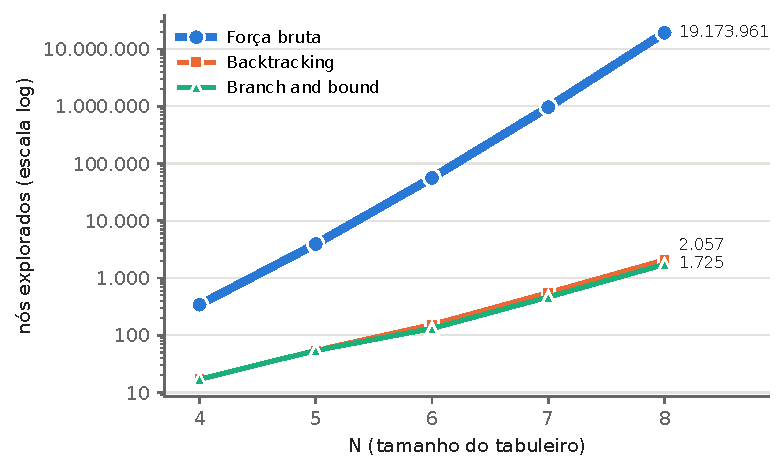
\includegraphics[width=\linewidth]{nos-rainhas.pdf}
\caption{Nós explorados pelos algoritmos de busca nas instâncias de N Rainhas, em função de N.}
\label{fig:nos-rainhas}
\end{figure}

A Tabela~\ref{tab:podas-rainhas} discrimina as podas por coluna, diagonal e limite; a Figura~\ref{fig:podas-rainhas} apresenta essas contagens graficamente. Para N=8, o Backtracking registra 10.212 podas por coluna e 3.452 por diagonal. No Branch and Bound, são 4.996 podas por coluna, 1.864 por diagonal e 560 pelo limite, avaliado 1.633 vezes.

\begin{table}[H]
\centering
\caption{N rainhas: podas por causa.}
\label{tab:podas-rainhas}
\small
\begin{tabular}{rrrrrrr}
\toprule
 & \multicolumn{2}{c}{Backtracking} & \multicolumn{4}{c}{Branch and bound} \\
\cmidrule(lr){2-3}\cmidrule(lr){4-7}
N & Coluna & Diagonal & Coluna & Diagonal & Limite & Avaliações do limite \\
\midrule
4 & 28     & 16    & 18    & 10    & 4   & 15    \\
5 & 119    & 48    & 105   & 42    & 4   & 44    \\
6 & 538    & 204   & 242   & 126   & 44  & 127   \\
7 & 2.239  & 794   & 1.151 & 444   & 130 & 424   \\
8 & 10.212 & 3.452 & 4.996 & 1.864 & 560 & 1.633 \\
\bottomrule
\end{tabular}
\end{table}

\begin{figure}[H]
\centering
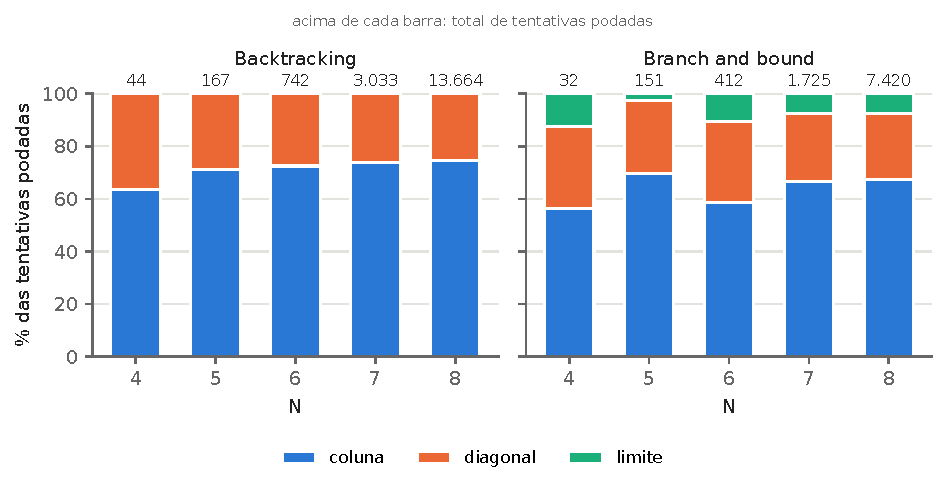
\includegraphics[width=\linewidth]{podas-rainhas.pdf}
\caption{Quantidade de podas por coluna, diagonal e limite nas instâncias de N Rainhas.}
\label{fig:podas-rainhas}
\end{figure}

A Tabela~\ref{tab:tsp} reúne o custo ótimo, os nós explorados e as rotas completas avaliadas para cada tamanho do TSP. Em n=10, força bruta e Backtracking exploram 986.410 nós e avaliam 181.440 rotas; o Branch and Bound explora 855 nós e avalia 11 rotas. A Figura~\ref{fig:nos-tsp} mostra os nós explorados em função do número de cidades.

\begin{table}[H]
\centering
\caption{Caixeiro-Viajante: custo ótimo, nós explorados e rotas completas avaliadas.}
\label{tab:tsp}
\small
\setlength{\tabcolsep}{4pt}
\begin{tabular}{rrrrrrrr}
\toprule
 & & \multicolumn{3}{c}{Nós explorados} & \multicolumn{3}{c}{Rotas avaliadas} \\
\cmidrule(lr){3-5}\cmidrule(lr){6-8}
n & Custo ótimo & FB & BT & B\&B & FB & BT & B\&B \\
\midrule
4  & 259 & 16      & 16      & 7   & 3       & 3       & 1  \\
6  & 138 & 326     & 326     & 41  & 60      & 60      & 3  \\
8  & 265 & 13.700  & 13.700  & 436 & 2.520   & 2.520   & 13 \\
10 & 233 & 986.410 & 986.410 & 855 & 181.440 & 181.440 & 11 \\
\bottomrule
\end{tabular}
\end{table}

\begin{figure}[H]
\centering
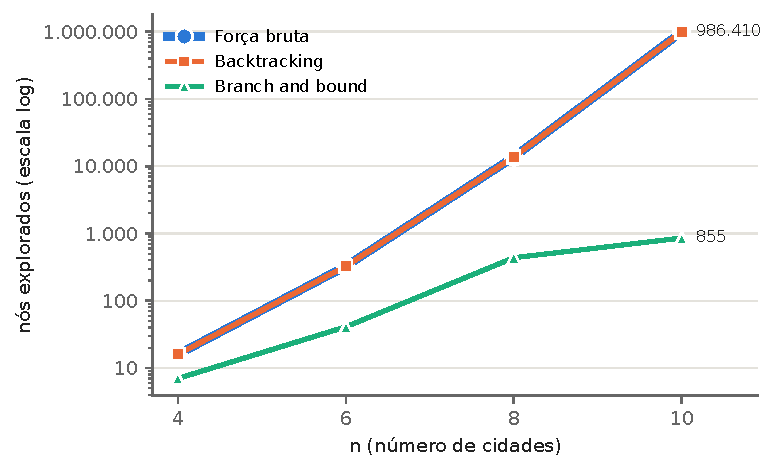
\includegraphics[width=\linewidth]{nos-tsp.pdf}
\caption{Nós explorados pelos algoritmos de busca nas instâncias do TSP, em função do número de cidades.}
\label{fig:nos-tsp}
\end{figure}

A Tabela~\ref{tab:tempo} apresenta a mediana, em milissegundos, de cinco execuções após a execução de aquecimento. Para N=8, os tempos são 175,0 ms para força bruta, 0,100 ms para Backtracking e 0,158 ms para Branch and Bound. Para n=10 no TSP, são 19,0 ms, 15,2 ms e 0,499 ms, respectivamente. As Figuras~\ref{fig:tempo-rainhas} e~\ref{fig:tempo-tsp} apresentam as medições por tamanho para cada problema.

\begin{table}[H]
\centering
\caption{Tempo de execução com aquecimento (mediana de 5 execuções, após 1 de aquecimento), em ms.}
\label{tab:tempo}
\begin{tabular}{lrrrr}
\toprule
Problema & Tamanho & Força bruta & Backtracking & Branch and bound \\
\midrule
N rainhas & 4  & 0,087 & 0,009 & 0,019 \\
N rainhas & 5  & 0,191 & 0,026 & 0,062 \\
N rainhas & 6  & 2,23  & 0,119 & 0,048 \\
N rainhas & 7  & 9,92  & 0,096 & 0,148 \\
N rainhas & 8  & 175,0 & 0,100 & 0,158 \\
\midrule
TSP       & 4  & 0,004 & 0,004 & 0,007 \\
TSP       & 6  & 0,096 & 0,083 & 0,069 \\
TSP       & 8  & 0,708 & 0,886 & 0,320 \\
TSP       & 10 & 19,0  & 15,2  & 0,499 \\
\bottomrule
\end{tabular}
\end{table}

\begin{figure}[H]
\centering
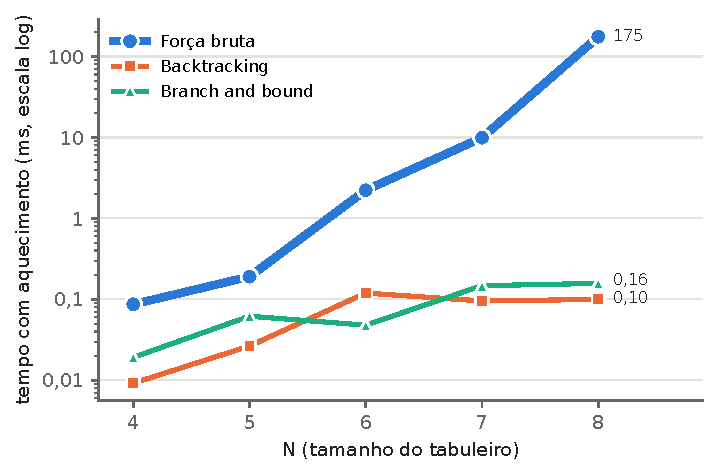
\includegraphics[width=\linewidth]{tempo-rainhas.pdf}
\caption{Tempo de execução dos algoritmos nas instâncias de N Rainhas; mediana de cinco execuções após aquecimento, em milissegundos.}
\label{fig:tempo-rainhas}
\end{figure}

\begin{figure}[H]
\centering
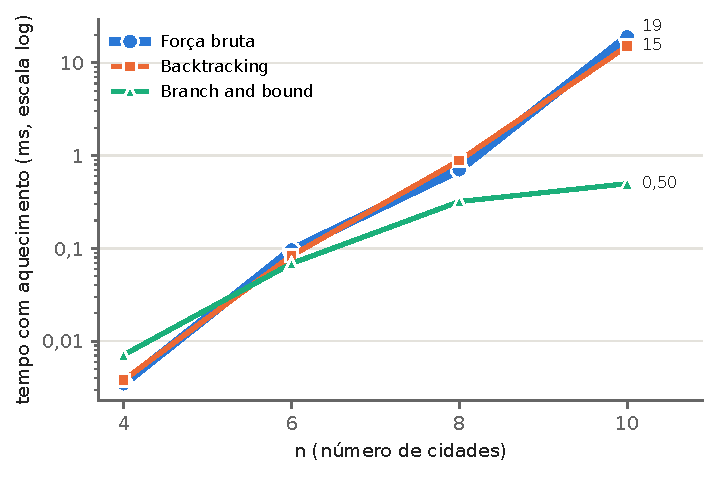
\includegraphics[width=\linewidth]{tempo-tsp.pdf}
\caption{Tempo de execução dos algoritmos nas instâncias do TSP; mediana de cinco execuções após aquecimento, em milissegundos.}
\label{fig:tempo-tsp}
\end{figure}

As Tabelas~\ref{tab:frio-rainhas} e~\ref{tab:frio-tsp} comparam o tempo da execução inicial registrada separadamente com a mediana das cinco execuções posteriores e apresentam a razão entre os valores. Nas N Rainhas, a maior razão da tabela é 50,7 para força bruta em N=4; no TSP, a razão para Branch and Bound em n=10 é 1,0. A Figura~\ref{fig:frio-aquecido} reúne essa comparação para os dois problemas.

\begin{table}[H]
\centering
\caption{N rainhas: tempo sem aquecimento (1 execução) e com aquecimento (mediana de 5), em ms, e a razão entre eles.}
\label{tab:frio-rainhas}
\small
\setlength{\tabcolsep}{3pt}
\begin{tabular}{rrrrrrrrrr}
\toprule
 & \multicolumn{3}{c}{Força bruta} & \multicolumn{3}{c}{Backtracking} & \multicolumn{3}{c}{Branch and bound} \\
\cmidrule(lr){2-4}\cmidrule(lr){5-7}\cmidrule(lr){8-10}
N & sem & com & razão & sem & com & razão & sem & com & razão \\
\midrule
4 & 4,40  & 0,087 & 50,7$\times$ & 0,056 & 0,009 & 6,1$\times$ & 0,059 & 0,019 & 3,1$\times$ \\
5 & 0,363 & 0,191 & 1,9$\times$  & 0,042 & 0,026 & 1,6$\times$ & 0,075 & 0,062 & 1,2$\times$ \\
6 & 6,03  & 2,23  & 2,7$\times$  & 0,131 & 0,119 & 1,1$\times$ & 0,118 & 0,048 & 2,5$\times$ \\
7 & 11,3  & 9,92  & 1,1$\times$  & 0,112 & 0,096 & 1,2$\times$ & 0,198 & 0,148 & 1,3$\times$ \\
8 & 191,1 & 175,0 & 1,1$\times$  & 0,139 & 0,100 & 1,4$\times$ & 0,200 & 0,158 & 1,3$\times$ \\
\bottomrule
\end{tabular}
\end{table}

\begin{table}[H]
\centering
\caption{Caixeiro-Viajante: tempo sem aquecimento (1 execução) e com aquecimento (mediana de 5), em ms, e a razão entre eles.}
\label{tab:frio-tsp}
\small
\setlength{\tabcolsep}{3pt}
\begin{tabular}{rrrrrrrrrr}
\toprule
 & \multicolumn{3}{c}{Força bruta} & \multicolumn{3}{c}{Backtracking} & \multicolumn{3}{c}{Branch and bound} \\
\cmidrule(lr){2-4}\cmidrule(lr){5-7}\cmidrule(lr){8-10}
n & sem & com & razão & sem & com & razão & sem & com & razão \\
\midrule
4  & 0,007 & 0,004 & 2,1$\times$ & 0,012 & 0,004 & 3,2$\times$ & 0,018 & 0,007 & 2,6$\times$ \\
6  & 0,095 & 0,096 & 1,0$\times$ & 0,102 & 0,083 & 1,2$\times$ & 0,079 & 0,069 & 1,2$\times$ \\
8  & 0,734 & 0,708 & 1,0$\times$ & 0,899 & 0,886 & 1,0$\times$ & 0,361 & 0,320 & 1,1$\times$ \\
10 & 28,6  & 19,0  & 1,5$\times$ & 15,9  & 15,2  & 1,0$\times$ & 0,501 & 0,499 & 1,0$\times$ \\
\bottomrule
\end{tabular}
\end{table}

\begin{figure}[H]
\centering
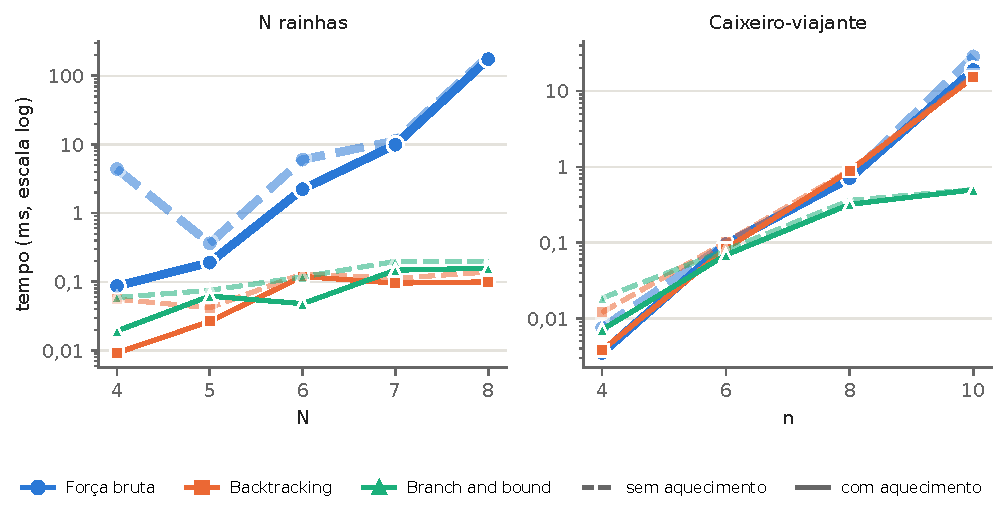
\includegraphics[width=\linewidth]{frio-aquecido.pdf}
\caption{Comparação entre o tempo da execução inicial registrada e a mediana de cinco execuções posteriores, para N Rainhas e TSP.}
\label{fig:frio-aquecido}
\end{figure}

\section{Discussão}

Nas N Rainhas, o Backtracking reduziu os nós explorados de 19.173.961 para 2.057 em N=8, em comparação com a força bruta, que enumera $N^N$ configurações. O Branch and Bound visitou ainda menos nós: 1.725 em N=8 e 464 em N=7. Essa redução, porém, não garantiu menor tempo: em N=7 e N=8, o B\&B levou 0,148 ms e 0,158 ms, contra 0,096 ms e 0,100 ms do Backtracking. Em N=6, foi mais rápido (0,048 ms contra 0,119 ms). O custo quadrático do limite por nó ajuda a explicar por que a redução de estados nem sempre compensa em tempo.

No TSP, força bruta e Backtracking exploraram a mesma quantidade de nós nos tamanhos avaliados. Em n=10, o Branch and Bound reduziu os nós de 986.410 para 855 e as rotas avaliadas de 181.440 para 11; seu tempo foi 0,499 ms, aproximadamente 38 vezes menor que os 19,0 ms da força bruta. Apesar desse resultado, o pior caso permanece fatorial: o limite baseado em árvore geradora mínima custa $O(n^2)$ por nó e pode não podar subárvores. Esse limite é o usado neste estudo e difere do método de Little et al., que prioriza a expansão pelo menor limite.

Os resultados ilustram que o efeito da poda depende do problema e do custo de suas verificações: nas N Rainhas, Backtracking já elimina estados que violam restrições; no TSP, a redução expressiva de nós observada veio com o limite do B\&B. Assim, a quantidade de nós, isoladamente, não determina o tempo de execução.

A análise é limitada pelos tamanhos pequenos, por uma única máquina e por uma instância simétrica por tamanho no TSP. Tempos abaixo de aproximadamente 0,1 ms também variaram entre medições; por exemplo, o Backtracking das N Rainhas registrou 0,119 ms em N=6 e 0,096 ms em N=7. Diferenças pequenas nesse intervalo devem ser interpretadas com cautela. A execução inicial foi registrada separadamente da mediana das cinco execuções posteriores, sem que o experimento avaliasse a causa da diferença.
% =====================================================================
\section{Conclusão}
% MATERIAL: limitações — tamanhos pequenos (P5), uma máquina (notebook),
% uma instância por tamanho no TSP.

Este estudo analisou como diferentes estratégias de poda afetam o desempenho de algoritmos de busca nas N Rainhas e no Problema do Caixeiro-Viajante. Os resultados indicam que esse efeito depende do problema e do custo das verificações: nas N Rainhas, o Backtracking reduziu substancialmente os nós explorados, enquanto o limite adicional do Branch and Bound nem sempre resultou em menor tempo. No TSP, o Branch and Bound reduziu os nós e as rotas avaliadas e apresentou o menor tempo nas instâncias consideradas. Assim, os experimentos respondem à questão de pesquisa mostrando que a poda pode melhorar o desempenho, mas a redução do espaço de busca, isoladamente, não garante menor tempo de execução.

Essas conclusões são limitadas pelos tamanhos pequenos avaliados, pela execução em uma única máquina e pelo uso de uma única instância simétrica por tamanho no TSP. Como continuidade, recomenda-se ampliar os tamanhos de entrada, testar diferentes instâncias do TSP e repetir a avaliação em outros ambientes computacionais, para verificar se os comportamentos observados se mantêm em condições mais variadas.

% =====================================================================
% Estilo de referências do template SBC (autor-data). Só as 4 aprovadas.
% Se alguma não for citada com \cite no texto, ela não aparece na lista;
% o \nocite abaixo garante as 4 enquanto o texto não estiver pronto.
\nocite{laaksonen:2018,haralick:1980,cormen:2012,little:1963}
\bibliographystyle{sbc}
\bibliography{referencias}

\end{document}
